\documentclass[11pt]{article}
\usepackage{minted, tikz}
\usepackage{amsfonts, amssymb, amsmath, float, tabularx}
\usepackage{enumerate, esint, nicefrac, algorithm2e}
\parindent 0px
\date{September 13, 2023}
\title{CS301 :: Homework 1}
\author{Ryan Magdaleno}
\begin{document}
\maketitle

%%%%%%%%%%%%%%%%%%%%%%%%%%%%%%%%%%%%%%%%%%%%%%%%%%%%%%%%%%%%%%%%%%%%%%%%%%%%%%%%%%%%%%%%%

\textbf{Problem 1. DFAs} 
\begin{enumerate}[a)]
\item
Generate the state diagram for a DFA which decides the following \\language $L$.
$\sum = \{0, 1\}.$ \\
$L = \{w\in\sum^*$ : $w$ does not start with $'00'$ and $w$ ends with $'01'$ \}


\vspace{5px}\textbf{Solution ::}
\begin{center}
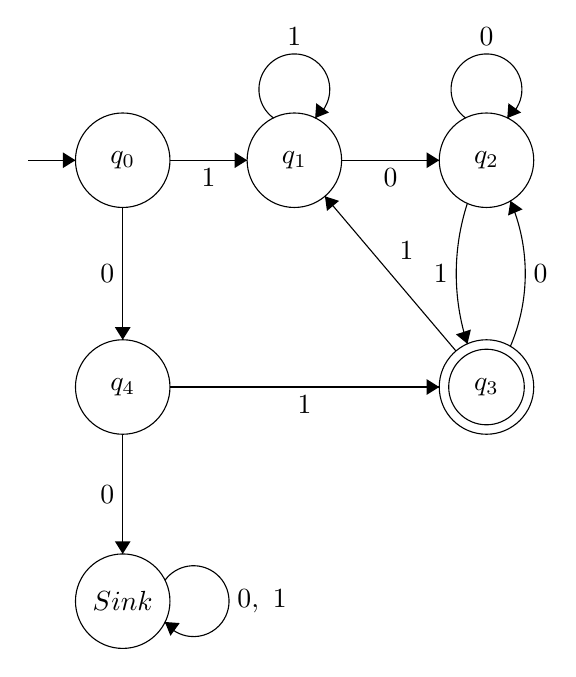
\begin{tikzpicture}[scale=0.2]
\tikzstyle{every node}+=[inner sep=0pt]
\draw [black] (14.7,-16.9) circle (3);
\draw (14.7,-16.9) node {$q_0$};
\draw [black] (25.6,-16.9) circle (3);
\draw (25.6,-16.9) node {$q_1$};
\draw [black] (37.8,-16.9) circle (3);
\draw (37.8,-16.9) node {$q_2$};
\draw [black] (37.8,-31.3) circle (3);
\draw (37.8,-31.3) node {$q_3$};
\draw [black] (37.8,-31.3) circle (2.4);
\draw [black] (14.7,-31.3) circle (3);
\draw (14.7,-31.3) node {$q_4$};
\draw [black] (14.7,-44.9) circle (3);
\draw (14.7,-44.9) node {$Sink$};
\draw [black] (17.7,-16.9) -- (22.6,-16.9);
\fill [black] (22.6,-16.9) -- (21.8,-16.4) -- (21.8,-17.4);
\draw (20.15,-17.4) node [below] {$1$};
\draw [black] (28.6,-16.9) -- (34.8,-16.9);
\fill [black] (34.8,-16.9) -- (34,-16.4) -- (34,-17.4);
\draw (31.7,-17.4) node [below] {$0$};
\draw [black] (36.585,-28.563) arc (-162.01501:-197.98499:14.454);
\fill [black] (36.59,-28.56) -- (36.81,-27.65) -- (35.86,-27.96);
\draw (35.38,-24.1) node [left] {$1$};
\draw [black] (17.7,-31.3) -- (34.8,-31.3);
\fill [black] (34.8,-31.3) -- (34,-30.8) -- (34,-31.8);
\draw (26.25,-31.8) node [below] {$1$};
\draw [black] (14.7,-34.3) -- (14.7,-41.9);
\fill [black] (14.7,-41.9) -- (15.2,-41.1) -- (14.2,-41.1);
\draw (14.2,-38.1) node [left] {$0$};
\draw [black] (17.38,-43.577) arc (144:-144:2.25);
\draw (21.95,-44.9) node [right] {$0,\mbox{ }1$};
\fill [black] (17.38,-46.22) -- (17.73,-47.1) -- (18.32,-46.29);
\draw [black] (14.7,-19.9) -- (14.7,-28.3);
\fill [black] (14.7,-28.3) -- (15.2,-27.5) -- (14.2,-27.5);
\draw (14.2,-24.1) node [left] {$0$};
\draw [black] (24.277,-14.22) arc (234:-54:2.25);
\draw (25.6,-9.65) node [above] {$1$};
\fill [black] (26.92,-14.22) -- (27.8,-13.87) -- (26.99,-13.28);
\draw [black] (35.86,-29.01) -- (27.54,-19.19);
\fill [black] (27.54,-19.19) -- (27.67,-20.12) -- (28.44,-19.48);
\draw (32.25,-22.66) node [right] {$1$};
\draw [black] (39.316,-19.479) arc (23.13951:-23.13951:11.759);
\fill [black] (39.32,-19.48) -- (39.17,-20.41) -- (40.09,-20.02);
\draw (40.76,-24.1) node [right] {$0$};
\draw [black] (36.477,-14.22) arc (234:-54:2.25);
\draw (37.8,-9.65) node [above] {$0$};
\fill [black] (39.12,-14.22) -- (40,-13.87) -- (39.19,-13.28);
\draw [black] (8.7,-16.9) -- (11.7,-16.9);
\fill [black] (11.7,-16.9) -- (10.9,-16.4) -- (10.9,-17.4);
\end{tikzpicture}
\end{center}
\pagebreak

\item
Give the 5-tuple which represents the DFA from 1a). You may use a table to 
represent the transition function $\delta$.

\vspace{5px}\textbf{Solution ::}

\begin{align*}
    Q &= \{q_0, q_1, q_2, q_3, q_4, q_5\} \\
    \sum &= \{0, 1\} \\
    q_0 &= q_0 \\
    F &= \{q_4\} \\
    \delta &=
    \begin{tabularx}{0.3\textwidth} { 
        | >{\centering\arraybackslash}X 
        | >{\centering\arraybackslash}X 
        | >{\centering\arraybackslash}X | }
        \hline & 0 & 1 \\
        \hline $q_0$ & $q_4$  & $q_1$  \\
        \hline $q_1$ & $q_2$  & $q_1$  \\
        \hline $q_2$ & $q_2$  & $q_3$  \\
        \hline $q_3$ & $q_2$  & $q_1$  \\
        \hline $q_4$ & $sink$  & $q_3$  \\
        \hline $sink$ & $sink$  & $sink$  \\
        \hline
    \end{tabularx}
\end{align*}
\end{enumerate}
\pagebreak

%%%%%%%%%%%%%%%%%%%%%%%%%%%%%%%%%%%%%%%%%%%%%%%%%%%%%%%%%%%%%%%%%%%%%%%%%%%%%%%%%%%%%%%%%

\textbf{Problem 2. NFAs}

\begin{enumerate}[a)]
\item 
Generate the state-diagram for an NFA which decides the following \\language $L$.
$\sum = \{0, 1\}$.
$$L = (010)^*\cup1^*(00)^*$$
\vspace{5px}\textbf{Solution ::}
\begin{center}
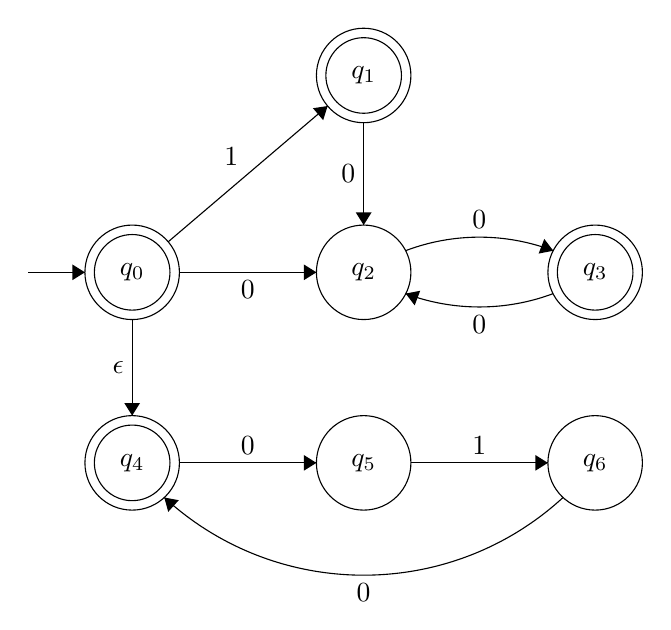
\begin{tikzpicture}[scale=0.2]
\tikzstyle{every node}+=[inner sep=0pt]
\draw [black] (15,-18.8) circle (3);
\draw (15,-18.8) node {$q_0$};
\draw [black] (15,-18.8) circle (2.4);
\draw [black] (29.7,-6.3) circle (3);
\draw (29.7,-6.3) node {$q_1$};
\draw [black] (29.7,-6.3) circle (2.4);
\draw [black] (29.7,-18.8) circle (3);
\draw (29.7,-18.8) node {$q_2$};
\draw [black] (44.4,-18.8) circle (3);
\draw (44.4,-18.8) node {$q_3$};
\draw [black] (44.4,-18.8) circle (2.4);
\draw [black] (15,-30.9) circle (3);
\draw (15,-30.9) node {$q_4$};
\draw [black] (15,-30.9) circle (2.4);
\draw [black] (29.7,-30.9) circle (3);
\draw (29.7,-30.9) node {$q_5$};
\draw [black] (44.4,-30.9) circle (3);
\draw (44.4,-30.9) node {$q_6$};
\draw [black] (8.4,-18.8) -- (12,-18.8);
\fill [black] (12,-18.8) -- (11.2,-18.3) -- (11.2,-19.3);
\draw [black] (18,-18.8) -- (26.7,-18.8);
\fill [black] (26.7,-18.8) -- (25.9,-18.3) -- (25.9,-19.3);
\draw (22.35,-19.3) node [below] {$0$};
\draw [black] (32.36,-17.427) arc (110.80093:69.19907:13.207);
\fill [black] (41.74,-17.43) -- (41.17,-16.68) -- (40.81,-17.61);
\draw (37.05,-16.07) node [above] {$0$};
\draw [black] (41.73,-20.155) arc (-69.52082:-110.47918:13.377);
\fill [black] (32.37,-20.15) -- (32.94,-20.9) -- (33.29,-19.97);
\draw (37.05,-21.5) node [below] {$0$};
\draw [black] (29.7,-9.3) -- (29.7,-15.8);
\fill [black] (29.7,-15.8) -- (30.2,-15) -- (29.2,-15);
\draw (29.2,-12.55) node [left] {$0$};
\draw [black] (17.29,-16.86) -- (27.41,-8.24);
\fill [black] (27.41,-8.24) -- (26.48,-8.38) -- (27.13,-9.14);
\draw (21.29,-12.06) node [above] {$1$};
\draw [black] (15,-21.8) -- (15,-27.9);
\fill [black] (15,-27.9) -- (15.5,-27.1) -- (14.5,-27.1);
\draw (14.5,-24.85) node [left] {$\epsilon$};
\draw [black] (18,-30.9) -- (26.7,-30.9);
\fill [black] (26.7,-30.9) -- (25.9,-30.4) -- (25.9,-31.4);
\draw (22.35,-30.4) node [above] {$0$};
\draw [black] (32.7,-30.9) -- (41.4,-30.9);
\fill [black] (41.4,-30.9) -- (40.6,-30.4) -- (40.6,-31.4);
\draw (37.05,-30.4) node [above] {$1$};
\draw [black] (42.363,-33.098) arc (-47.4198:-132.5802:18.715);
\fill [black] (17.04,-33.1) -- (17.29,-34.01) -- (17.96,-33.27);
\draw (29.7,-38.53) node [below] {$0$};
\end{tikzpicture}
\end{center}
\pagebreak

\item 
Give the 5-tuple which represents the NFA from 2a). You may use a table to represent
the transition function $\delta$.
\begin{align*}
    Q &= \{q_0, q_1, q_2, q_3, q_4, q_5, q_6\} \\
    \sum &= \{0, 1\} \\
    q_0 &= q_0 \\
    F &= \{q_0,q_1,q_3,q_4\} \\
    \delta &=
    \begin{tabularx}{0.5\textwidth} { 
        | >{\centering\arraybackslash}X 
        | >{\centering\arraybackslash}X 
        | >{\centering\arraybackslash}X 
        | >{\centering\arraybackslash}X | }
        \hline & 0 & 1 & $\epsilon$\\
        \hline $q_0$ & \{$q_2$\} & \{$q_1$\} & \{$q_4$\} \\
        \hline $q_1$ & \{$q_2$\} & \{$q_1$\} & $\O$ \\
        \hline $q_2$ & \{$q_3$\} & $\O$ & $\O$ \\
        \hline $q_3$ & \{$q_2$\} & $\O$ & $\O$ \\
        \hline $q_4$ & \{$q_5$\} & $\O$ & $\O$ \\
        \hline $q_5$ & $\O$ & \{$q_6$\} & $\O$ \\
        \hline $q_6$ & \{$q_4$\} & $\O$ & $\O$ \\
        \hline
    \end{tabularx}
\end{align*}
\end{enumerate}
\pagebreak

%%%%%%%%%%%%%%%%%%%%%%%%%%%%%%%%%%%%%%%%%%%%%%%%%%%%%%%%%%%%%%%%%%%%%%%%%%%%%%%%%%%%%%%%%

\textbf{Problem 3. Closure} 

Given the 5-tuple for an NFA $M_L = (Q, \sum, \delta, q_0, F)$ which decides, $L$,
\\describe how to produce the 5-tuple for an NFA $M_{L^R} = (Q_R, \sum, \delta_R,
q_{0_R}, F_R)$ which decides $L^R$, the reverse of $L$.


\vspace{10px}\textit{The reverse, $L^R$ is the recursive operation given below which
gives the reverse of a string.}

$e.g.\,\, (110)^R=011$
\begin{itemize}
    \item $\epsilon^R=\epsilon$
    \item For string $w$ and character $a, (wa)^R=a(w^R)$
\end{itemize}
\vspace{5px}\textbf{Solution ::}
\begin{align*}
    Q^R &= Q \\
    \sum^R &= \sum \\
    q_{0^R} &= F \\
    F^R &= q_0
\end{align*}
For the transition function let's use the following string example:\\
$L={1011}, L^R$ should become ${1011}$.
\begin{center}
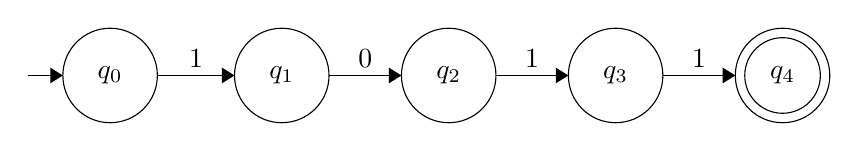
\begin{tikzpicture}[scale=0.2]
\tikzstyle{every node}+=[inner sep=0pt]
\draw [black] (12.6,-24.2) circle (3);
\draw (12.6,-24.2) node {$q_0$};
\draw [black] (23.5,-24.2) circle (3);
\draw (23.5,-24.2) node {$q_1$};
\draw [black] (34.1,-24.2) circle (3);
\draw (34.1,-24.2) node {$q_2$};
\draw [black] (44.7,-24.2) circle (3);
\draw (44.7,-24.2) node {$q_3$};
\draw [black] (55.3,-24.2) circle (3);
\draw (55.3,-24.2) node {$q_4$};
\draw [black] (55.3,-24.2) circle (2.4);
\draw [black] (15.6,-24.2) -- (20.5,-24.2);
\fill [black] (20.5,-24.2) -- (19.7,-23.7) -- (19.7,-24.7);
\draw (18.05,-23.7) node [above] {$1$};
\draw [black] (26.5,-24.2) -- (31.1,-24.2);
\fill [black] (31.1,-24.2) -- (30.3,-23.7) -- (30.3,-24.7);
\draw (28.8,-23.7) node [above] {$0$};
\draw [black] (37.1,-24.2) -- (41.7,-24.2);
\fill [black] (41.7,-24.2) -- (40.9,-23.7) -- (40.9,-24.7);
\draw (39.4,-23.7) node [above] {$1$};
\draw [black] (47.7,-24.2) -- (52.3,-24.2);
\fill [black] (52.3,-24.2) -- (51.5,-23.7) -- (51.5,-24.7);
\draw (50,-23.7) node [above] {$1$};
\draw [black] (7.4,-24.2) -- (9.6,-24.2);
\fill [black] (9.6,-24.2) -- (8.8,-23.7) -- (8.8,-24.7);
\end{tikzpicture}
\end{center}

$L$ transition function $\delta:$

\begin{center}
\begin{tabularx}{0.3\textwidth} { 
    | >{\centering\arraybackslash}X 
    | >{\centering\arraybackslash}X 
    | >{\centering\arraybackslash}X | }
    \hline & 1 & 0 \\
    \hline $q_0$ & $q_1$ & $\O$ \\
    \hline $q_1$ & $\O$ & $q_1$ \\
    \hline $q_2$ & $q_3$ & $\O$ \\
    \hline $q_3$ & $q_4$ & $\O$ \\
    \hline $q_4$ & $\O$ & $\O$ \\
    \hline
\end{tabularx}
\end{center}
\pagebreak

To retrieve the string we need to invert the starting and final state. \\
(As noted with $q_{0^R}=F$, $F^R=q_0$). After that we must reverse the transition
function of $L; \delta$.

One method to reverse $\delta$ would be to enter the original starting state, in
this example $q_0$, and enter each state sort of recursively, so we go:
$$q_0\rightarrow q_1\rightarrow q_2\rightarrow q_3$$
and stop when the next state only has the empty set on all transitions, this would
be our base case.

In this example we wold stop at $q_3$ because $q_4$ terminates fully. We can now
reverse and in the end the $L^R$ transition function $\delta^R$ should look like this:

\begin{center}
    \begin{tabularx}{0.3\textwidth} { 
        | >{\centering\arraybackslash}X 
        | >{\centering\arraybackslash}X 
        | >{\centering\arraybackslash}X | }
        \hline & 1 & 0 \\
        \hline $q_0$ & $\O$ & $\O$ \\
        \hline $q_1$ & $q_0$ & $\O$ \\
        \hline $q_2$ & $\O$ & $q_1$ \\
        \hline $q_3$ & $q_2$ & $\O$ \\
        \hline $q_4$ & $q_3$ & $\O$ \\
        \hline
    \end{tabularx}
    \end{center}
The final NFA $L^R$ should now be reverse in all strings cases like so:
\begin{center}
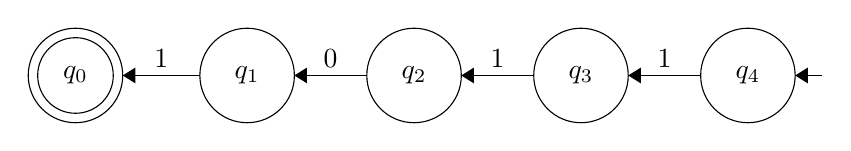
\begin{tikzpicture}[scale=0.2]
\tikzstyle{every node}+=[inner sep=0pt]
\draw [black] (12.6,-24.2) circle (3);
\draw (12.6,-24.2) node {$q_0$};
\draw [black] (12.6,-24.2) circle (2.4);
\draw [black] (23.5,-24.2) circle (3);
\draw (23.5,-24.2) node {$q_1$};
\draw [black] (34.1,-24.2) circle (3);
\draw (34.1,-24.2) node {$q_2$};
\draw [black] (44.7,-24.2) circle (3);
\draw (44.7,-24.2) node {$q_3$};
\draw [black] (55.3,-24.2) circle (3);
\draw (55.3,-24.2) node {$q_4$};
\draw [black] (52.3,-24.2) -- (47.7,-24.2);
\fill [black] (47.7,-24.2) -- (48.5,-24.7) -- (48.5,-23.7);
\draw (50,-23.7) node [above] {$1$};
\draw [black] (41.7,-24.2) -- (37.1,-24.2);
\fill [black] (37.1,-24.2) -- (37.9,-24.7) -- (37.9,-23.7);
\draw (39.4,-23.7) node [above] {$1$};
\draw [black] (31.1,-24.2) -- (26.5,-24.2);
\fill [black] (26.5,-24.2) -- (27.3,-24.7) -- (27.3,-23.7);
\draw (28.8,-23.7) node [above] {$0$};
\draw [black] (20.5,-24.2) -- (15.6,-24.2);
\fill [black] (15.6,-24.2) -- (16.4,-24.7) -- (16.4,-23.7);
\draw (18.05,-23.7) node [above] {$1$};
\draw [black] (60,-24.2) -- (58.3,-24.2);
\fill [black] (58.3,-24.2) -- (59.1,-24.7) -- (59.1,-23.7);
\end{tikzpicture}
\end{center}

Extra note: Doing the steps listed above again should result in the original $L$,
that is:
$$L={(L^R)}^R$$

\end{document}